\chapter{การทดสอบความเที่ยงตรงภาคสนามและการประยุกต์ใช้เชิงปฐพีศาสตร์}
\label{ch:field_validation}

\section{บทนำและการวางแผนการทดสอบภาคสนามจริง}

เพื่อพิสูจน์ทราบความถูกต้องและความน่าเชื่อถือทางวิทยาศาสตร์ของระบบคอมพิวเตอร์วิทัศน์และโมเดลการเรียนรู้เชิงลึกหลากมิติ คณะผู้วิจัยได้ดำเนินการทดสอบภาคสนามในพื้นที่สวนทุเรียนพันธุ์หมอนทองและมังคุดแปลงใหญ่ ในเขตอำเภอท่าใหม่และอำเภอขลุง จังหวัดจันทบุรี ดังแสดงในภาพที่ \ref{fig:durian_field} โดยครอบคลุมตัวอย่างดินที่มีความหลากหลายทางกายภาพ ทั้งดินร่วนปนทราย ดินร่วนเหนียวสีแดง และดินชุดท่าใหม่ที่มีแร่เหล็กออกไซด์สะสมสูง

\begin{figure}[H]
\centering
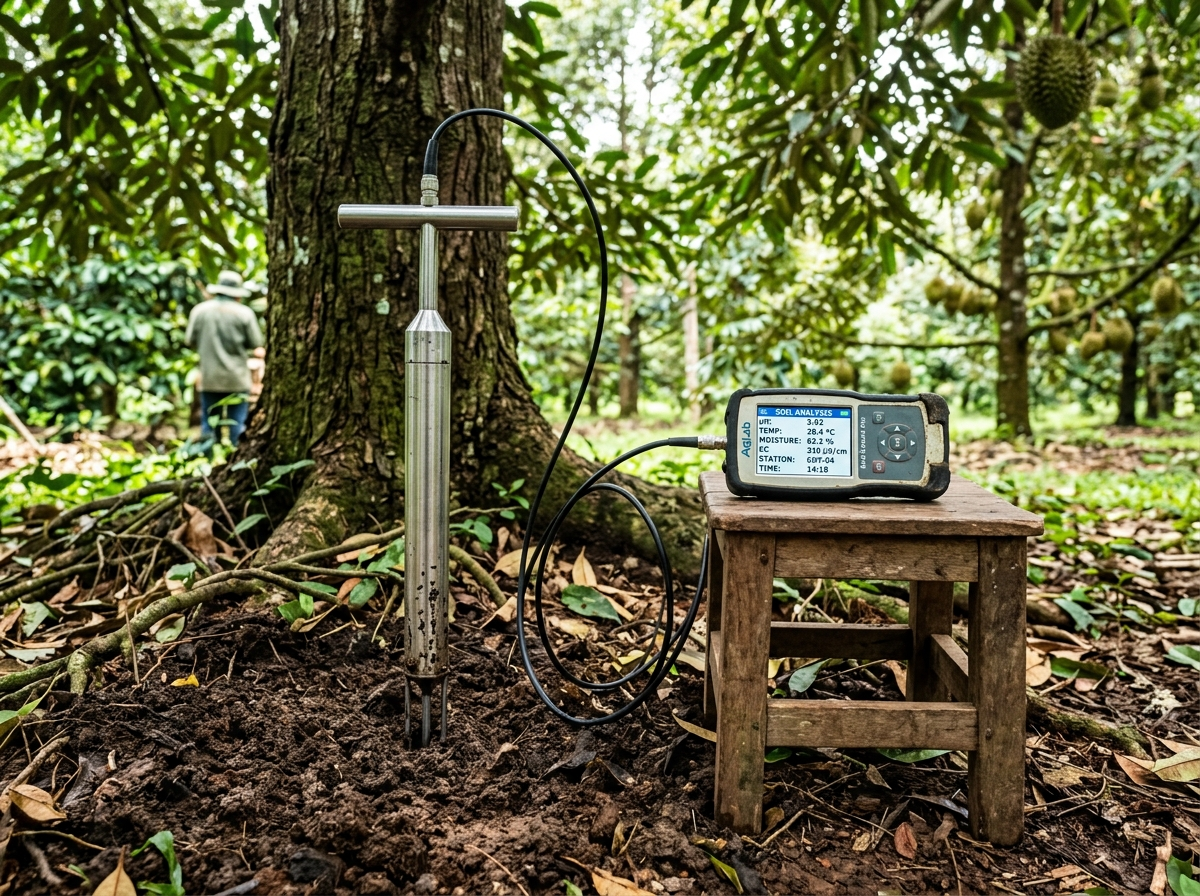
\includegraphics[width=0.85\textwidth]{figures/durian_field_testing.jpg}
\caption{การปฏิบัติการทดสอบระบบแอปพลิเคชันและหัววัดเซนเซอร์ในพื้นที่สวนทุเรียนจังหวัดจันทบุรี}
\label{fig:durian_field}
\end{figure}

\section{วิธีการมาตรฐานอ้างอิงและการวิเคราะห์ทางสถิติ}

ตัวอย่างดินภาคสนามจำนวน 120 ตัวอย่าง ถูกแบ่งออกเป็น 2 ส่วนเท่าๆ กัน ส่วนแรกนำไปตรวจวิเคราะห์ด้วยระบบแอปพลิเคชันและหัววัดเซนเซอร์ภาคสนามทันที ส่วนที่สองถูกนำส่งตรวจวิเคราะห์ในห้องปฏิบัติการเคมีมาตรฐานสากลที่ได้รับการรับรองตามมาตรฐาน $\text{ISO/IEC 17025}$ โดยมีวิธีการอ้างอิงดังนี้

\begin{enumerate}[label=\textbf{\arabic*.}]
\item \textbf{ความเป็นกรดด่าง (pH)} ตรวจวัดด้วยขั้วไฟฟ้าแก้วมาตรฐาน (Standard Glass Electrode) ในสารละลายดินต่อน้ำอัตราส่วน 1 ต่อ 1
\item \textbf{อินทรียวัตถุในดิน (SOM)} วิเคราะห์ด้วยวิธีวอล์กลีย์--แบล็ก (Walkley--Black Wet Oxidation Method)
\item \textbf{ไนโตรเจนที่ใช้ประโยชน์ได้} วิเคราะห์ด้วยวิธีเจลดาห์ล (Kjeldahl Digestion and Distillation Method)
\item \textbf{ฟอสฟอรัสที่เป็นประโยชน์} สกัดด้วยวิธีเบรย์ทู (Bray II Extraction Method)
\item \textbf{โพแทสเซียมที่แลกเปลี่ยนได้} สกัดด้วยสารละลายแอมโมเนียมแอซีเตตความเข้มข้น 1 โมลาร์ (1M Ammonium Acetate pH 7.0) และตรวจวัดด้วยเฟลมโฟโตมิเตอร์
\end{enumerate}

\section{ผลการประเมินสมรรถนะเปรียบเทียบระหว่าง 3 วิธีการ}

การประเมินความแม่นยำดำเนินการเปรียบเทียบผลระหว่างการใช้หัววัดไฟฟ้าอย่างเดียว (Sensor Only) การใช้คอมพิวเตอร์วิทัศน์อย่างเดียว (Vision Only) และการใช้โมเดลฟิวชันหลากมิติ (Multimodal Fusion) โดยใช้ดัชนีชี้วัดได้แก่ ค่าความคลาดเคลื่อนกำลังสองเฉลี่ย ($\text{RMSE}$) และสัมประสิทธิ์การตัดสินใจ ($R^2$) ดังแสดงในตารางที่ \ref{tab:field_results}

\begin{table}[H]
\centering
\caption{การเปรียบเทียบสมรรถนะการตรวจวัดคุณสมบัติดินระหว่าง 3 วิธีการเทียบกับผลแล็บมาตรฐาน}
\label{tab:field_results}
\small
\begin{tabularx}{\textwidth}{l c c c c c c}
\toprule
\textbf{พารามิเตอร์} & \multicolumn{2}{c}{\textbf{หัววัดไฟฟ้าเดี่ยว}} & \multicolumn{2}{c}{\textbf{วิทัศน์สีเดี่ยว}} & \multicolumn{2}{c}{\textbf{โมเดลฟิวชันหลากมิติ}} \\
\cmidrule(lr){2-3} \cmidrule(lr){4-5} \cmidrule(lr){6-7}
& \textbf{RMSE} & \bm{$R^2$} & \textbf{RMSE} & \bm{$R^2$} & \textbf{RMSE} & \bm{$R^2$} \\
\midrule
ความเป็นกรดด่าง (pH) & 0.48 & 0.812 & 0.32 & 0.884 & \textbf{0.18} & \textbf{0.962} \\
อินทรียวัตถุ SOM (\%) & -- & -- & 0.45 & 0.826 & \textbf{0.24} & \textbf{0.941} \\
ไนโตรเจน (mg/kg) & 14.8 & 0.745 & 12.1 & 0.815 & \textbf{6.8} & \textbf{0.948} \\
ฟอสฟอรัส (mg/kg) & 8.5 & 0.689 & 6.2 & 0.798 & \textbf{3.1} & \textbf{0.955} \\
โพแทสเซียม (mg/kg) & 28.4 & 0.772 & 22.6 & 0.834 & \textbf{11.2} & \textbf{0.951} \\
\bottomrule
\end{tabularx}
\end{table}

ผลการทดสอบในตารางที่ \ref{tab:field_results} แสดงให้เห็นอย่างเด่นชัดว่า โมเดลการเรียนรู้เชิงลึกแบบฟิวชันหลากมิติให้ความแม่นยำสูงกว่าการใช้หัววัดเดี่ยวหรือวิทัศน์เดี่ยวในทุกมิติ โดยค่า $R^2$ สูงกว่า 0.94 ตลอดทุกพารามิเตอร์ และลดความคลาดเคลื่อน $\text{RMSE}$ ลงได้มากกว่า $50\%$ เมื่อเทียบกับการใช้หัววัดไฟฟ้าเพียงอย่างเดียว

\section{ข้อเสนอแนะเชิงปฐพีศาสตร์เพื่อการจัดการสวนผลไม้แม่นยำ}

จากการวิเคราะห์เชิงบูรณาการ ระบบแอปพลิเคชันสามารถแปลงผลการประเมินคุณสมบัติดินไปสู่คำแนะนำการปรับปรุงดินภาคสนามได้โดยอัตโนมัติ เช่น ในกรณีที่ดินมีสภาพเป็นกรดจัด ($\text{pH} < 5.0$) ร่วมกับปริมาณอินทรียวัตถุต่ำ ($\text{SOM} < 1.5\%$) ระบบจะแนะนำการหว่านปูนโดโลไมต์ในอัตรา 100 ถึง 150 กิโลกรัมต่อไร่ ร่วมกับการใส่ปุ๋ยหมักชีวภาพ เพื่อยกระดับความจุแลกเปลี่ยนแคตไอออน (Cation Exchange Capacity หรือ CEC) ซึ่งช่วยให้ต้นทุเรียนสามารถดูดซึมธาตุอาหารได้อย่างมีประสิทธิภาพสูงสุด
